\section{Methodology}
\label{sec:intro:methodology}

A research strategy has been defined in order to achieve the statement and derived goals presented
in Section \ref{sec:intro:hypothesis}. The strategy is defined as follows:

\begin{enumerate}
    \item Update knowledge by reviewing the literature in the area of activity modelling and recognition, knowledge engineering, machine learning and data mining. This analysis has been reinforced by attending specialised scientific conferences.
    \item Critically evaluate existing activity modelling and recognition solutions, analysing their scope and limitations and identifying weak areas where contributions to the state of the art can be done.
    \item Design and develop the different modules of the activity model learner, incrementally adopting more complex and efficient solutions.
    \item Test developed modules through experiments and analyse results to enhance the performance of the system.
    \item Attend conferences and workshops to present partial results and validate them with the scientific community.
    \item Experimentation and evaluation of the prototype at each particular stage.
    \item Network with experts at conferences, project meetings and consortia (the author is an active member of the SONOPA project\footnote{http://www.sonopa.eu/} - SOcial Networks for Older adults to Promote an Active Life -). Contact for particular details by e-mail or by visiting other research groups (the author was a visiting researcher in De Montfort University for 6 weeks in 2014).
    \item Redesign the activity model learner system with feedback from all this network, as well as the literature.
    \item Select an appropriate evaluation methodology and evaluate consequently the activity model learner system.
    \item Dissemination of the results obtained during the research process.
\end{enumerate}

This methodology is illustrated in \myfig{fig-methodology}, as a cyclic process which starts with the review of the state of the art and finishes with the publications and the final prototype.

\begin{figure}[htbp]
\centering
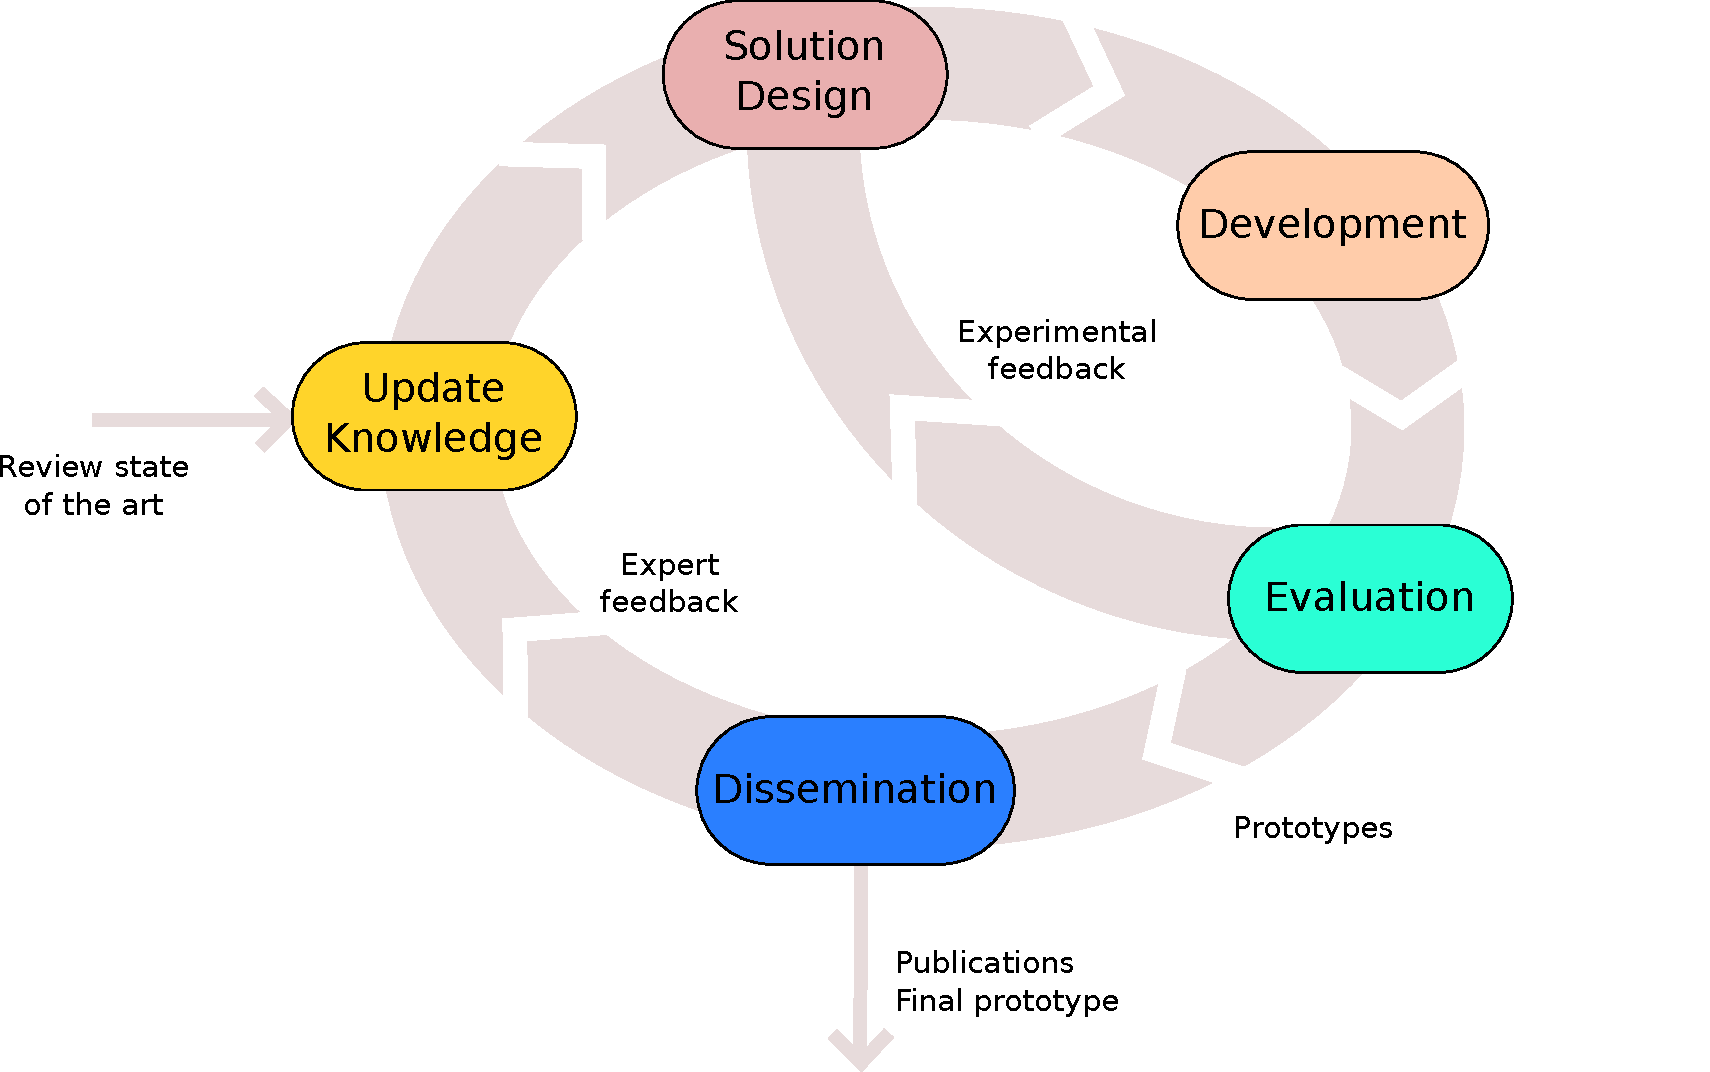
\includegraphics[width=\textwidth]{ball_methodology.pdf}
    \caption{Followed research methodology.}
    \label{fig-methodology}
\end{figure}


